%----------------------------------------------------------------------------------------
%	SECTION 1.5
%----------------------------------------------------------------------------------------

\section{The Subspace Topology.}

\begin{theorem}\label{1.5.1}
    Let $X$ be a topological space with topology $\Tc$, and let $Y \subseteq X$. Then the
    collection:
        \begin{equation*}
            \Tc_y = \{Y \cap U: U \in \Tc\}
        \end{equation*}
    forms a topology on $Y$.
\end{theorem}
\begin{proof}
    Cleary, $Y \cap \emptyset=\emptyset \in \Tc_Y$ and  $Y \cap X=Y \in \Tc_Y$. Now  consider the collection
    $\{U_{\alpha}\}$. Then  $\bigcup{(Y \cap U_{\alpha})}=Y \cap \bigcup{U_{\alpha}}$, similarly, for  $\{U_i\}_{i=1}^n$,
    $\bigcap{(Y \cap U_i)}=Y \cap \bigcap{U_i}$, hence  $\Tc$ is a topology on  $Y$.
\end{proof}

\begin{definition}
    Let $X$ be a topological space, and let  $Y \subseteq X$. We call the $\Tc$ defined
    in theorem \ref{1.5.1} the \textbf{subspace topology} on $Y$. We say that $U \subseteq Y$ is
    \textbf{open in $Y$} if $U \in \Tc_Y$.
\end{definition}

\begin{lemma}\label{1.5.2}
    Let $\Bc$ be the basis for a topology on  $X$. Then the collection  $\Bc_Y=\{B \cap Y: B \in \Bc\}$,
    where  $Y \subseteq X$, is a basis for the subspace topology on  $Y$.
\end{lemma}
\begin{proof}
    Let $U$ be open in  $X$, and let  $y \in Y \cap U$, and choose  $B \in \Bc$ such that
    $y \in B \subseteq U$, then  $y \in B \cap Y \subseteq U \cap Y$, then by lemma \ref{1.2.2},
     $\Bc_y$ is the basis fpr the subspace topology on  $Y$.
\end{proof}

\begin{lemma}\label{1.5.3}
    Let $Y$ be a subspace of  $X$, If  $U \subseteq Y$ is open in  $Y$ and $Y$
    is open in  $X$, then  $U$ is open in  $X$.
\end{lemma}
\begin{proof}
    Let $U \in \Tc_Y$, then for some  $V \subseteq X$,  $U=Y \cap V$. Now since  $Y$ is open in  $X$, and so
    is  $V$, then  it follows that $U$ is also open in  $X$.
\end{proof}
\begin{remark}
    What this lemma says is that given a topological space $X$, and a subspace  $Y$ of  $X$, then the
    subspace topology of  $Y$ is courser than the topology on  $X$, i.e.  $\Tc_Y \subseteq \Tc$.
\end{remark}

\begin{theorem}\label{1.5.4}
    If $A$ is a subspace of  $X$, and  $B$ is a subspace of  $Y$, then the product topology on
     $A \times B$ is the topology that  $A \times B$ inherits as a subspace of  $X \times Y$.
\end{theorem}
\begin{proof}
    We have that $U \times V$ is the basis element for $X \times Y$, with  $U$ open in  $X$, and
    $V$ open in  $Y$. Thus  $(U \times V) \cap (A \times B)=(U \cap A) \times (V \cap B)$ is a basis element
    for the subspace topology on $X \times Y$. Since  $U \cap A$ and  $V \cap B$ are open in the subspace
    topologies of  $A$ and  $B$ respectively, then  $(U  \cap A) \times (V \cap B)$ is a basis for
    the product topology on $A \times B$.
\end{proof}

\begin{example}
    \begin{enumerate}
        \item[(1)] Consider $[0,1] \subseteq \R$. In the subspace topology of  $[0,1]$, we have as
            basis elements of the form $(a,b) \cap [0,1]$, with $(a,b) \subseteq \R$. If we have
            that  $(a,b) \subseteq [0,1]$, then $(a,b) \cap [0,1]=(a,b)$. On the other hand, if $a \in [0,1]$
            or $b \in [0,1]$, then we get $(a,b) \cap [0,1]=(a,1]$ or $(a,b) \cap [0,1]=[0,b)$, lastly if neither
            $a$ nor  $b$ are in $[0,1]$, then we have $(a,b) \cap [0,1]=[0,1]$ only if  $[0,1] \subseteq (a,b)$, and
            $(a,b) \cap [0,1]=\emptyset$ otherwise.

            The only one of these sets open in $\R$ under the standard topology
            is $(0,1)$.

        \item[(2)] For  $[0,1) \cup \{2\} \subseteq \R$, the singletoun  $\{2\}$ is open in the
            subspace topology on $[0,1) \cup \{2\}$; for observe, that $(\frac{3}{5},\frac{5}{2}) \cap
            ([0,1) \cup \{2\})=\{2\}$, however, in the order topology, on that same set, $\{2\}$ is not open.
            Any basis element on  $[0,1) \cup \{2\}$ containing  $2$ is of the form $(a,2]$, where
            $a \in [0,1) \cup \{2\}$.

        \item[(3)] The dictionary order on $[0,1] \times [0,1]$ is a restriction of the dictionary order
            on $\R \times \R$. Now the set  $\{\frac{1}{2}\} \times (\frac{1}{2},1]$ is open in the
            subspace topology on $[0,1] \times [0,1]$, but it is not open in the dictionary order on the
            same set.
    \end{enumerate}
\end{example}

\begin{definition}
    We call the set $[0,1] \times [0,1]$ on the dictionary odere the \textbf{ordered square}, and we
    denote it by $I_0^2$.
\end{definition}

\begin{lemma}\label{1.5.5}
    Let $Y$ be a subspace of a topological space  $X$, and let  $A \subseteq
    Y$. Then the topology of  $A$ as a subspace of  $Y$ is the same as the
    topolgy of  $A$ as a subspace of  $X$.
\end{lemma}
\begin{proof}
    Let $V$ be open in  $Y$, then $V \cap A$ is open in $A$ as a subspace of
    $Y$, however, since $Y$ is a subspace of $X$,  $V=U \cap Y$ for some  $U$
    open in $X$, so $V \cap A=(U \cap Y) \cap A=U \cap (A \cap Y)=U \cap A$,
    making $V \cap A$ open in $A$ as a subspace of $X$.

    Conversely, if $U$ is open in $X$, then $U \cap A$ is open in $A$ as a
    subspace of $X$, additionally, $U \cap Y$ is open in  $Y$ as a subspace of
    $Y$, so that  $(U \cap Y) \cap A=U \cap (A \cap Y)=U \cap A$, which makes $U
    \cap A$ open in $A$ as a subspace of $Y$.
\end{proof}

\begin{example}\label{1.9}
    Suppose that $\Tc$ and  $\Tc'$ are topologies on a set $X$, with $\Tc
    \subseteq \Tc'$. Then if  $Y \subseteq X$, then the topology of  $Y$ as a
    subspace of  $X$ under  $\Tc'$ is finer than the topology of  $Y$ as a
    subspace of  $X$ under  $\Tc$; for, if  $U$ is open in  $X$ under  $\Tc$,
    then  $U \cap Y$ is open in  $Y$ under  $\Tc$. But  $\Tc \subseteq \Tc'$,
    which implies that  $U \cap Y$ is open in  $Y$ under  $\Tc'$
\end{example}

\begin{definition}
    Let $X$ be an ordered set. We say that a nonempty subset $Y \subset X$ is \textbf{convex}
    in $X$ if for each pair of points  $a,b \in Y$, with  $a<b$, then the open interval  $(a,b) \subseteq X$ is
    also contained in  $Y$.
\end{definition}

\begin{figure}[h]
    \centering
    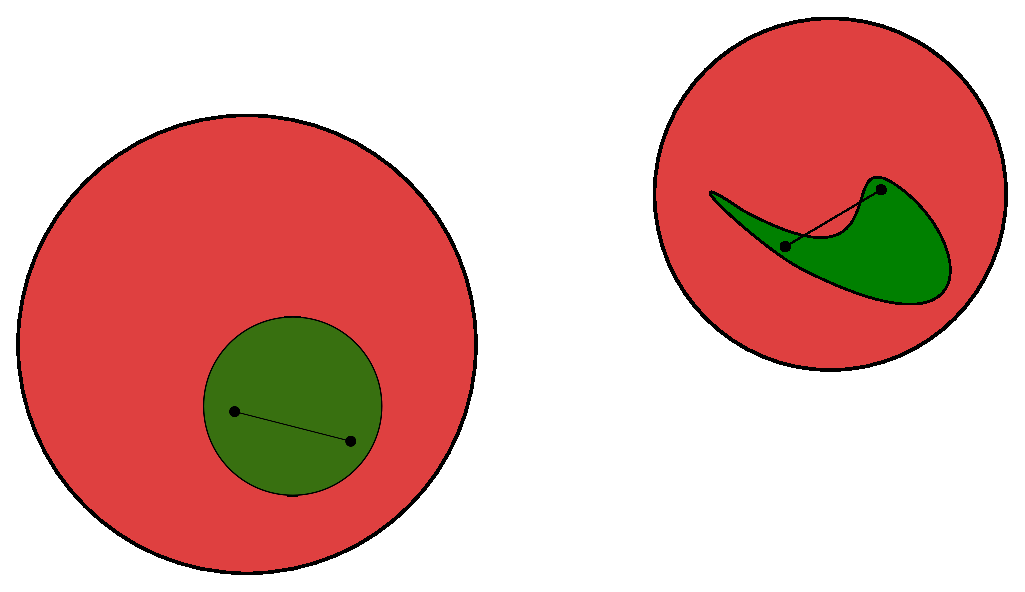
\includegraphics[scale = 0.5]{Figures/chapter1/convex_nonconvex.eps}
    \caption{A convex set, and a nonconvex set.}
    \label{fig1.6}
\end{figure}

\begin{example}
    Let $X$ be any ordered set. Then by definition, all open intervals and rays in
    $X$ are convex in  $X$.
\end{example}

\begin{theorem}\label{1.5.5}
    Let $X$ be an ordered set on the order toplogy, and let  $Y \subseteq X$ be convex in  $X$.
    Then the order topology on  $Y$ is the same as the subspace topology on  $Y$.
\end{theorem}
\begin{proof}
    Consider $(a, \infty) \subseteq X$. If  $a \in Y$, then  $(a,\infty) \cap Y=\{x \in Y: x>a\}$,
    which is by definition an open ray on $Y$. Now if  $a \notin Y$, then  $a$ is either a lowerbound, or
    an upperbound. Then  $(a, \infty) \cap Y=\emptyset$ and  $(-\infty,a) \cap Y=Y$ if  $a$ is an
    upperbound, similarly, if  $a$ is a lowerbound we get  $(a, \infty) \cap Y=Y$ and  $(-\infty,a) \cap Y=\emptyset$.

    Since $(a, \infty) \cap Y$ and  $(-\infty,a) \cap Y$ form a subbasis on the subspace topology on  $Y$,
    and since they are also open in  the order topology, then the order topology contains the subspace topology.

    Now if  $(a, \infty)$ is an open ray in  $Y$, then  $(a,\infty)=(b,\infty) \cap Y$, with $(b, \infty)$
    some open ray in  $X$, hence  $(a, \infty)$ is open in the subspace topology of  $Y$, and since
    it also forms the subbasis for the order topology, we have that the order
    topology is contained within the subspace topology. Thus both topologies are
    equal.
\end{proof}

\begin{figure}[h]
    \centering
    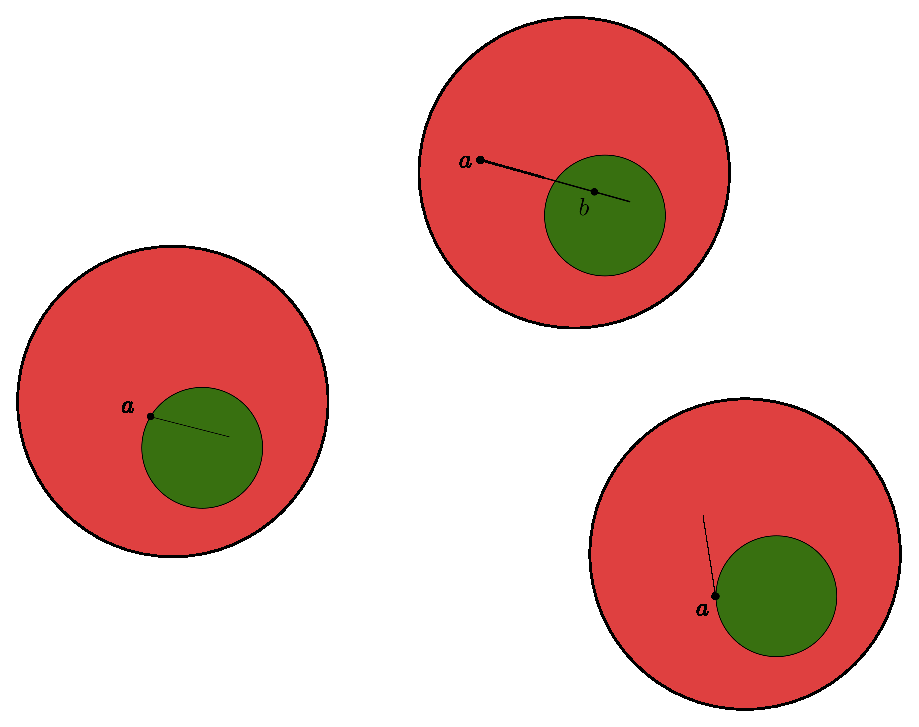
\includegraphics[scale = 0.5]{Figures/chapter1/thm_1_55.eps}
    \caption{An illustration of theorem \ref{1.5.5}.}
    \label{fig1.7}
\end{figure}

